\section{Séance 4}

\paragraph{1. } On considère un réseau de 5 villes. Le coût de la construction d'une route directe entre $i$ et $j$ est $A_{ij}$ avec $A$ donnée par~:
\[
  A = \begin{bmatrix}
    0 & 3 & 5 & 11 & 9 \\
    3 & 0 & 3 & 9 & 8 \\
    5 & 3 & 0 & +\infty & 10 \\
    11 & 9 & +\infty & 0 & 7 \\
    9 & 8 & 10 & 7 & 0
  \end{bmatrix}
\]
Trouvez le coût minimum d'un réseau liant les villes entre elles.

\paragraph{2. } Combien d'arbres différents à 5 sommets existe-t-il (avec ou sans symétrie)?

\paragraph{3. } Soit $T(G)$ le nombre d'arbres sous-tendants de $G$ et soit $e$ une arête du graphe $G$ qui n'est pas une boucle. La formule de Cayley établit la relation suivante~:
\[
  T(G) = T(G \backslash e) + T(G.e)
\]
où $G \backslash e$ est le graphe obtenu de $G$ en lui enlevant l'arête $e$ et $G.e$ est le graphe obtenu de $G \backslash e$ en fusionnant les extrémités de l'arête $e$. Appliquez la formule de Cayley au graphe suivant.

\begin{figure}[h!]
  \begin{center}
    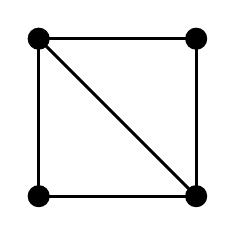
\begin{tikzpicture}[scale=1,looseness=1,auto,line width=.4mm]

      \draw (0,0) -- (0,2);
      \draw (0,2) -- (2,2);
      \draw (2,2) -- (2,0);
      \draw (2,0) -- (0,0);
      \draw (2,0) -- (0,2);

      \draw[fill=black] (0,0) circle(.12);
      \draw[fill=black] (0,2) circle(.12);
      \draw[fill=black] (2,2) circle(.12);
      \draw[fill=black] (2,0) circle(.12);

    \end{tikzpicture}
  \end{center}
\end{figure}
\vspace{-.5cm}

Combien d'arbres sous-tendants ce graphe possède-t-il?

\paragraph{4. } Considérons le graphe connexe $G = (V, E, \psi)$. Etant donné une partition $\Pi = \{V_1, V_2\}$ de $V$, On définit la \emph{coupe} $C(\Pi)$ de $G$ relative à $\Pi$ comme l'ensemble des arêtes de $G$ suivant~:
\[
  C(\Pi) := \{ (v_1, v_2) \in E : v_1 \in V_1 \text{ et } v_2 \in V_2 \}.
\]
Montrez qu'une coupe et un arbre sous-tendant de $G$ ont au moins une arête en commun.

\paragraph{5. } Montrez que si on veut trouver un arbre de recouvrement qui minimise l'arête la plus chère, il suffit de trouver l'arbre de poids minimum.

\paragraph{6. } Trouvez un graphe 3-connexe et 3-arête-connexe.

\paragraph{7. } L'identité suivante a été vue au cours~:
\[
  \text{connectivité } \leq \text{ arête-connectivité } \leq \text{ degré minimum}.
\]
Trouvez un graphe pour lequel les inégalités sont des égalités. Trouvez ensuite un graphe pour lequel les inégalités sont strictes.

\paragraph{8. } On définit $\delta$, $n$ et $k$ respectivement comme le degré minimum, le nombre de sommets et la connectivité d'un graphe simple $G$. Trouvez un graphe $G$ tel que $\delta = n-3$ et $k < \delta$.
